\documentclass{beamer}

\usetheme{default}
\usepackage[utf8]{inputenc}

\setbeamertemplate{footline}[frame number]
\setbeamertemplate{frametitle}[default][center]

\mode<presentation>{
\usetheme{Dresden}
%\setbeamercovered{transparent}
\usecolortheme{seagull}
}

\setbeamertemplate{headline}{}

\definecolor{peeblue}{RGB}{1,123,165}
\setbeamercolor*{palette primary}{fg=black,bg=peeblue!80}
\setbeamercolor*{palette secondary}{fg=black,bg=peeblue!80!gray!80}
\setbeamercolor*{palette tertiary}{fg=black,bg=peeblue!100}
\setbeamercolor*{palette quaternary}{fg=black,bg=peeblue!110}

\usebackgroundtemplate
{%
    \begin{picture}(210,40)(-5,2)
    
\includegraphics[width=0.07\paperwidth,keepaspectratio]{imgs/pee-logo-short.png}
    \end{picture}%
}

\title{Técnicas de Regularização em Aprendizado Profundo}
\author{Autor da Apresentação}
\date{\today}

\institute
{
  Universidade Federal do Rio de Janeiro\\
  UFRJ/COPPE/PEE
}


% Let's get started
\begin{document}

{
\usebackgroundtemplate{
    \begin{picture}(210,55)(-5,0)
    
\includegraphics[height=0.14\paperwidth,keepaspectratio]{imgs/pee-logo.png}
    \end{picture}%
    \begin{picture}(210,55)(-28,2)
    
\includegraphics[height=0.14\paperwidth,keepaspectratio]{imgs/coppe-logo.pdf}
    \end{picture}
}
\begin{frame}
  \bigskip\bigskip\bigskip\bigskip
  \titlepage
\end{frame}
}

\begin{frame}{Agenda}
  \tableofcontents
\end{frame}

\section{Introdução}

\begin{frame}{Introdução}
\end{frame}

\begin{frame}{Definição}
\begin{quote}
``Any modification we make to a learning algorithm that is intended to reduce its generalization error but not its training error.''
\end{quote}
\vspace{0.5cm}
\raggedleft
--- Goodfellow et al. Deep Learning
\end{frame}

\begin{frame}{Introdução: O Problema do Overfitting}
\centering
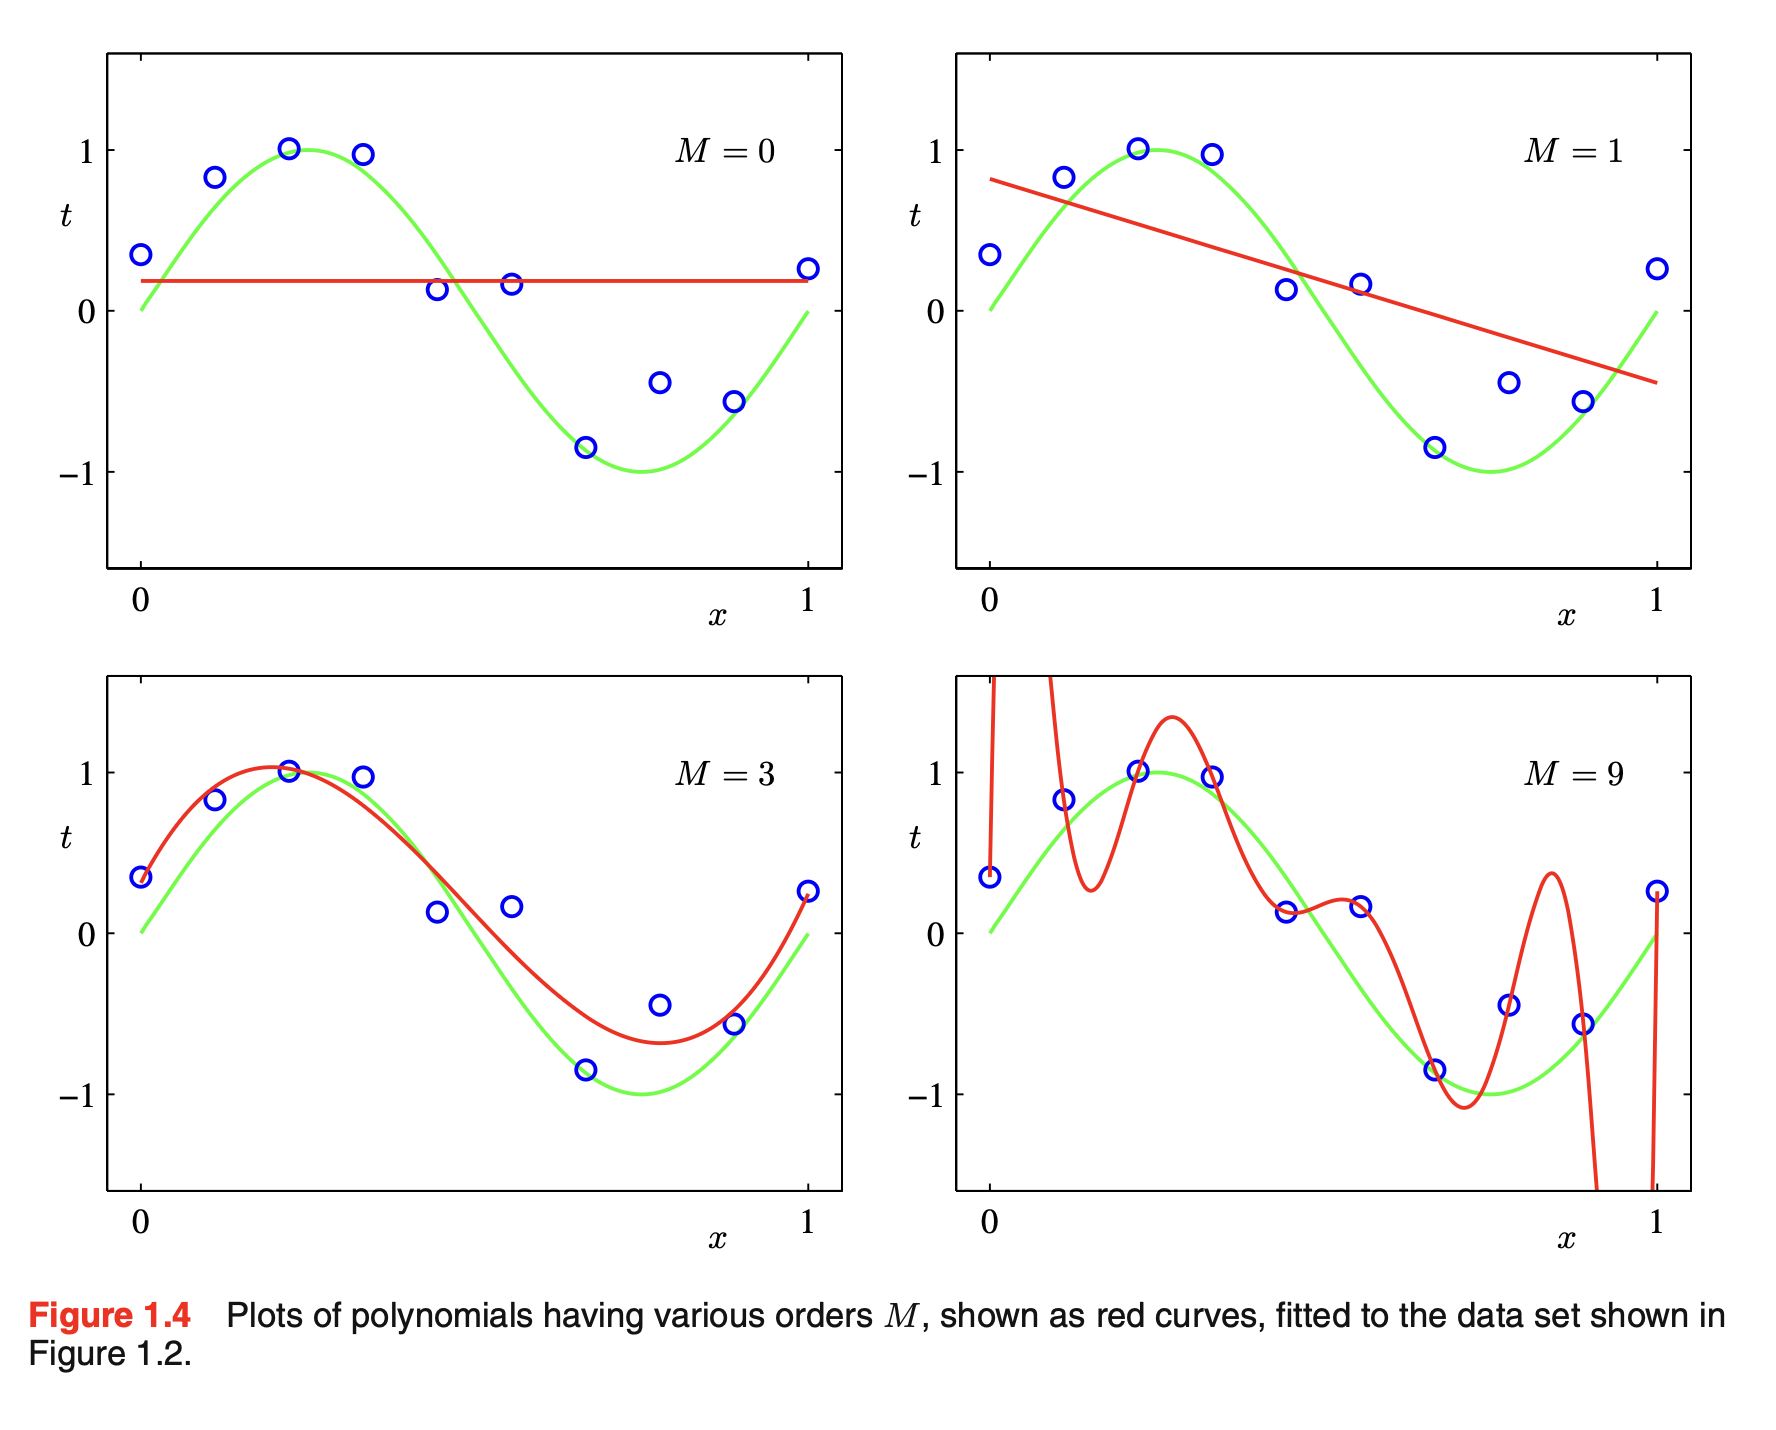
\includegraphics[width=\textwidth,height=0.8\textheight,keepaspectratio]{imgs/bishop_example/1.png}
\end{frame}

\begin{frame}
\centering
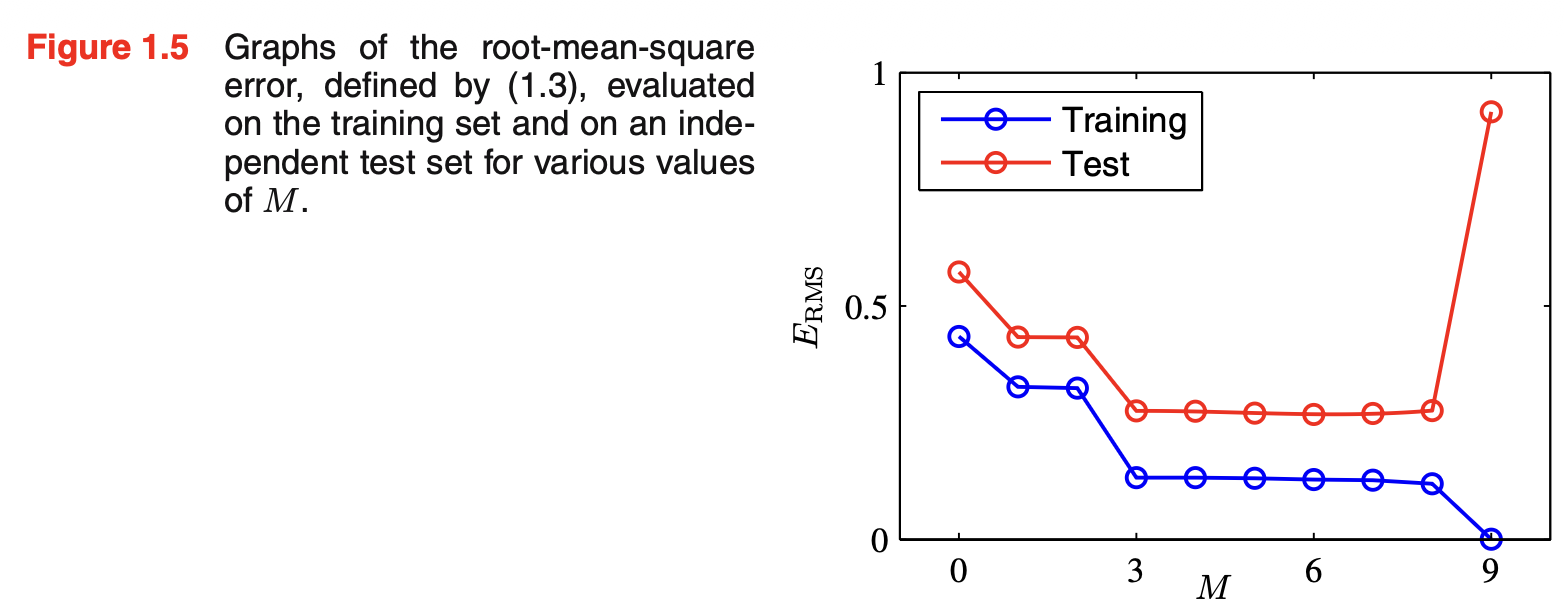
\includegraphics[width=\textwidth,height=0.8\textheight,keepaspectratio]{imgs/bishop_example/2.png}
\end{frame}

\begin{frame}{Alternativa 1: aumentar a quantidade de dados no treinamento}
\centering
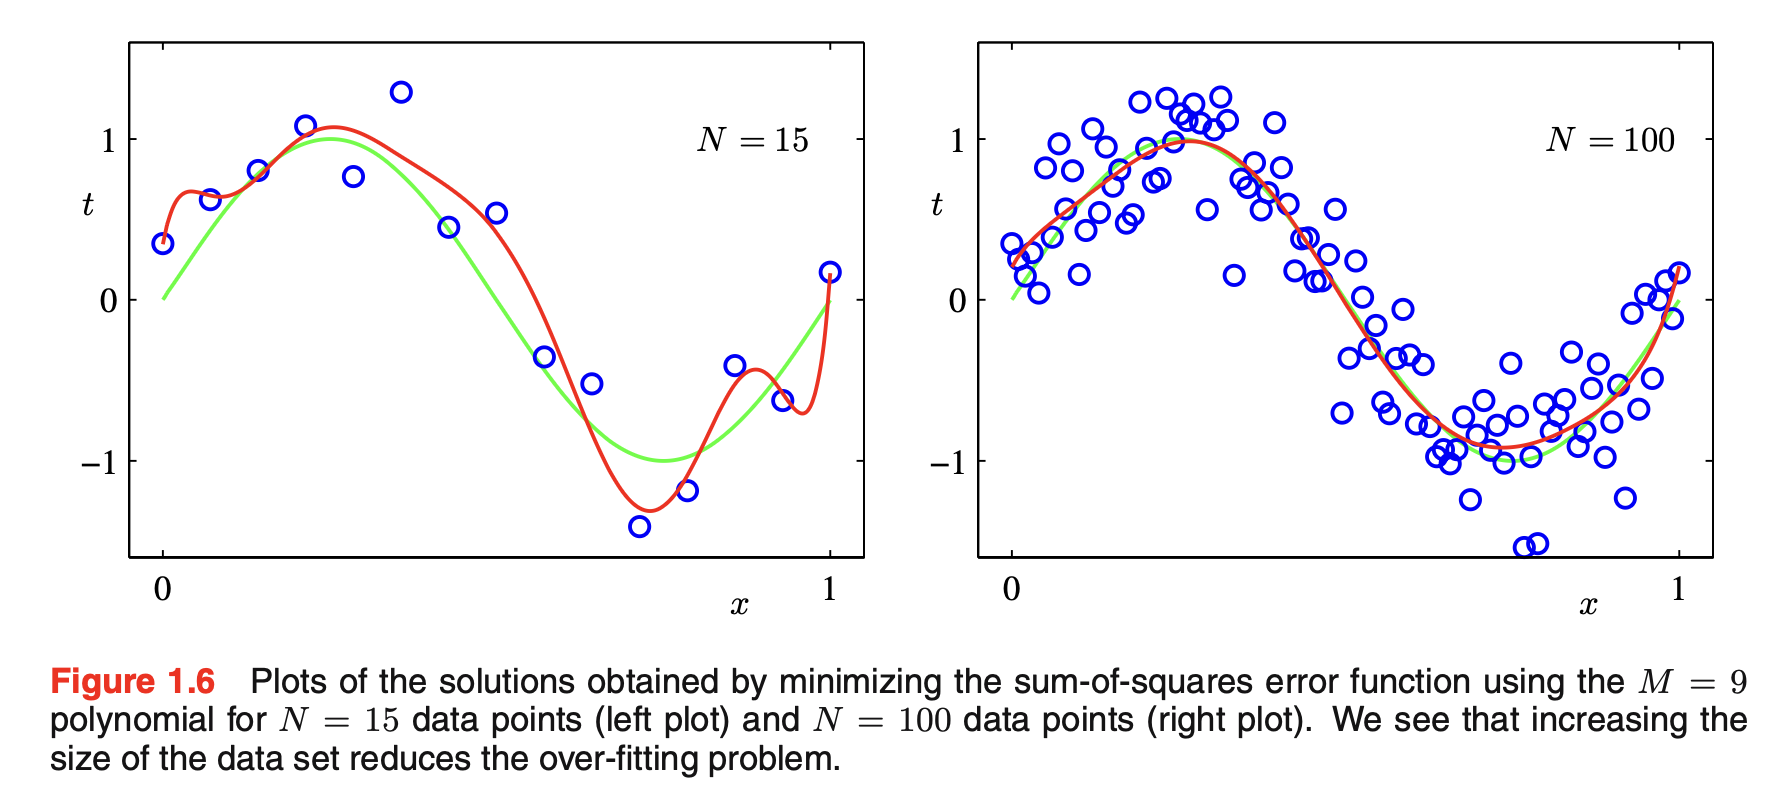
\includegraphics[width=\textwidth,height=0.8\textheight,keepaspectratio]{imgs/bishop_example/3.png}
Nem sempre é possível. Ex: Experimento genético com 500 pessoas, DNA humano tem de 19000 a 20000 genomas
\end{frame}

\begin{frame}{Alternativa 2: aplicar regularização}
\centering
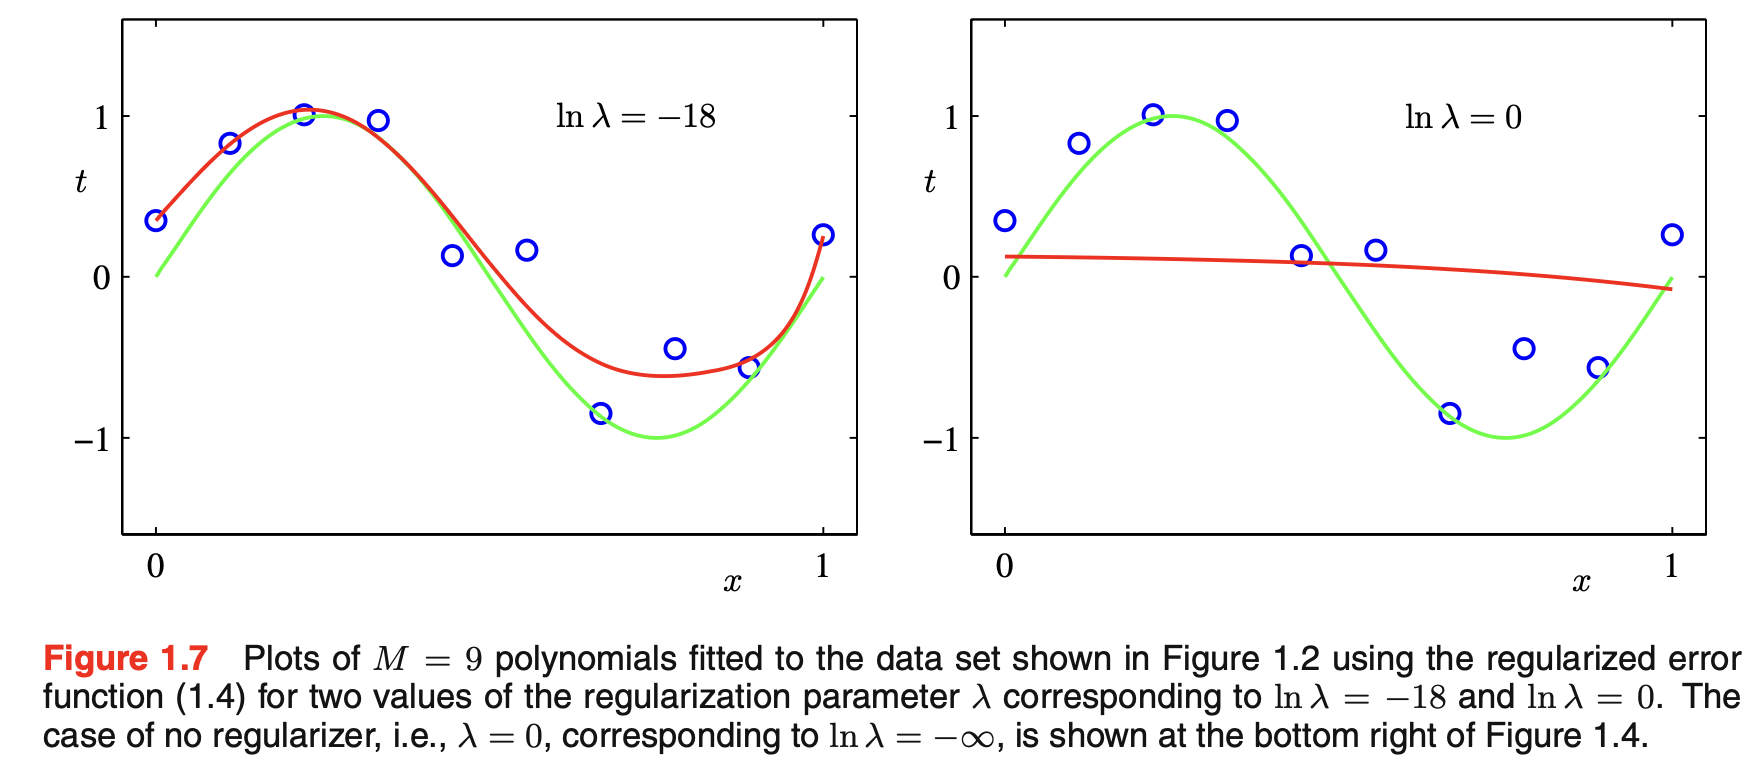
\includegraphics[width=\textwidth,height=0.8\textheight,keepaspectratio]{imgs/bishop_example/4.png}
\end{frame}

\begin{frame}
\centering
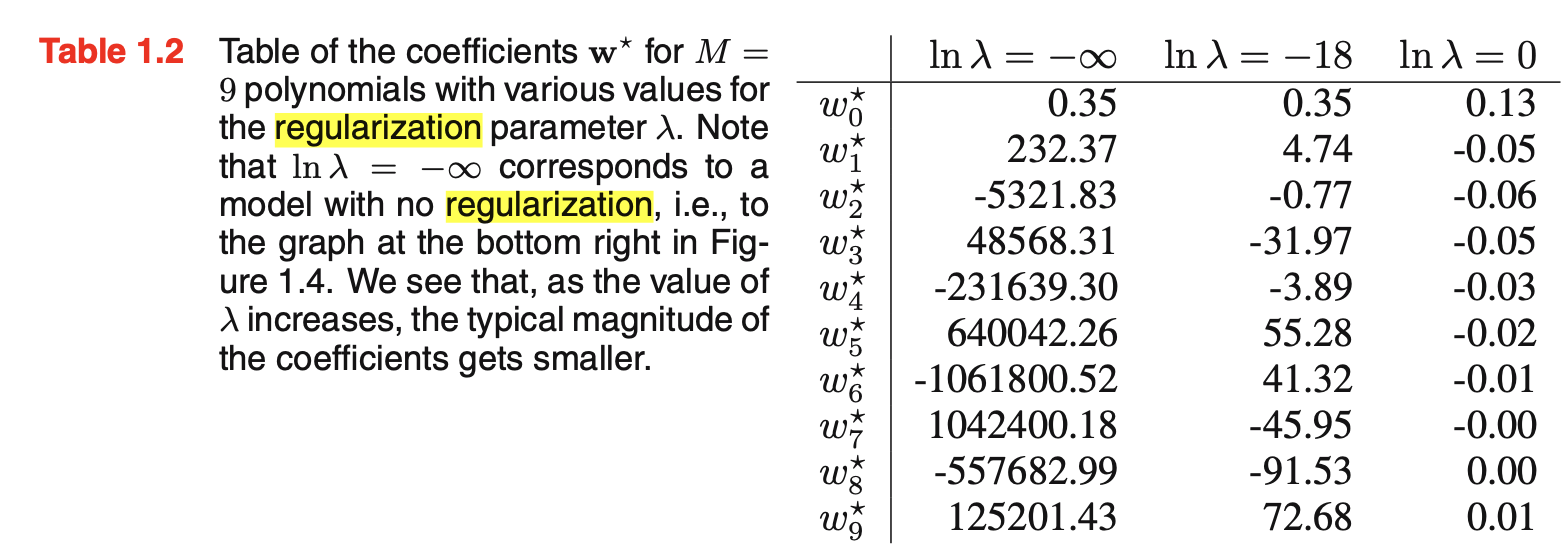
\includegraphics[width=\textwidth,height=0.8\textheight,keepaspectratio]{imgs/bishop_example/5.png}
\footnotesize{Na prática, o valor de $\lambda$ é obtido pela validação cruzada.}
\end{frame}

\section{Penalização da Norma dos Parâmetros}

\begin{frame}{Regularização L1 vs L2}
\begin{columns}[T]
\begin{column}{0.5\textwidth}
\begin{block}{Regularização L1}
\vspace{0.3cm}
{\tiny
$$\mathcal{L}(\theta) = \frac{1}{N}\sum_{i=1}^{N}\text{Custo}(y_i, f_\theta(x_i)) + \lambda||\theta||_1$$
}
\vspace{0.5cm}
- Pesos esparsos

- \textbf{exatamente zero}
\vspace{0.3cm}
\end{block}
\end{column}

\begin{column}{0.48\textwidth}
\begin{block}{Regularização L2}
\vspace{0.3cm}
{\tiny
$$\mathcal{L}(\theta) = \frac{1}{N}\sum_{i=1}^{N}\text{Custo}(y_i, f_\theta(x_i)) + \lambda||\theta||_2^2$$
}
\vspace{0.5cm}
- Pesos pequenos

- \textbf{nunca exatamente zero}
\vspace{0.3cm}
\end{block}
\end{column}
\end{columns}
\end{frame}


\begin{frame}{Interpretação Geométrica}
\centering
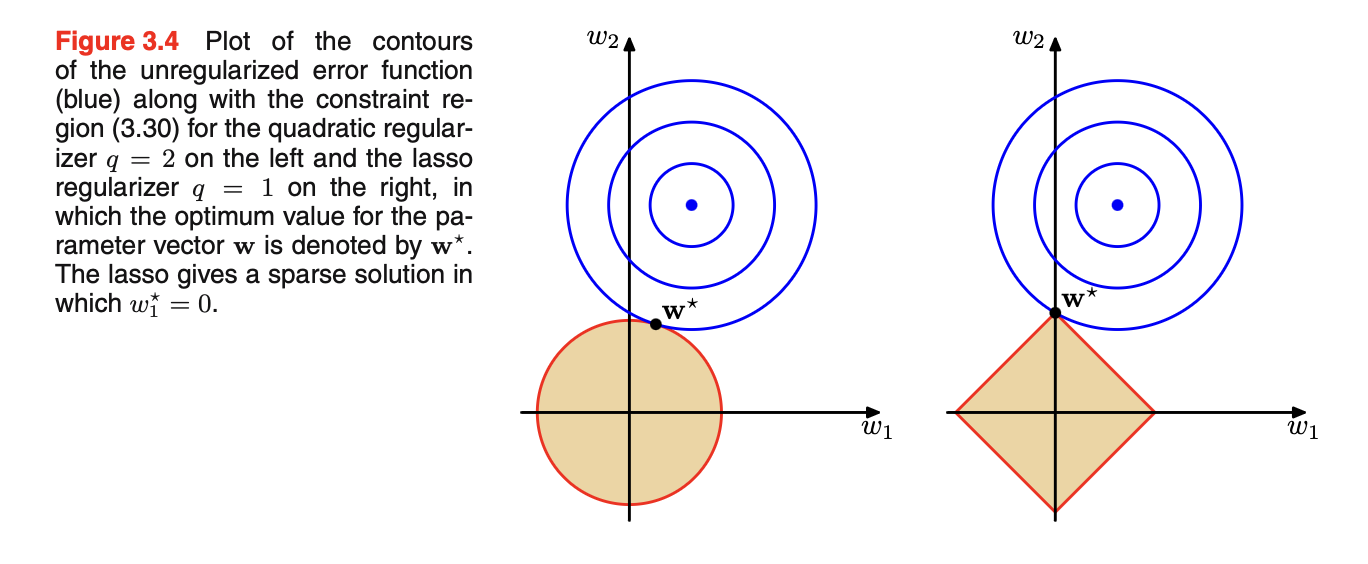
\includegraphics[width=\textwidth,height=0.8\textheight,keepaspectratio]{imgs/bishop_example/7.png}
\end{frame}

\section{Inductive Bias}

\begin{frame}{Inverse Problems}
\end{frame}

\begin{frame}{No Free Lunch Theorem}
\end{frame}

\begin{frame}{Symmetry and Invariance}
\end{frame}

\begin{frame}{Equivariance}
\end{frame}

\section{Weight Decay}

\begin{frame}{Consistent Regularizers}
\end{frame}

\begin{frame}{Generalized Weight Decay}
\end{frame}

\section{Learning Curves}

\begin{frame}{Early Stopping}
\end{frame}

\begin{frame}{Double Descent}
\end{frame}

\section{Parameter Sharing}

\begin{frame}{Soft Weight Sharing}
\end{frame}

\section{Residual Connections}

\begin{frame}{Residual Connections}
\end{frame}

\section{Model Averaging}

\begin{frame}{Dropout}
\end{frame}

\section{Regularization for Deep Learning (Goodfellow)}

\begin{frame}{Parameter Norm Penalties}
\end{frame}

\begin{frame}{Norm Penalties as Constrained Optimization}
\end{frame}

\begin{frame}{Regularization and Under-Constrained Problems}
\end{frame}

\begin{frame}{Dataset Augmentation}
\end{frame}

\begin{frame}{Noise Robustness}
\end{frame}

\begin{frame}{Semi-Supervised Learning}
\end{frame}

\begin{frame}{Multi-Task Learning}
\end{frame}

\begin{frame}{Parameter Tying and Parameter Sharing}
\end{frame}

\begin{frame}{Sparse Representations}
\end{frame}

\begin{frame}{Bagging and Other Ensemble Methods}
\end{frame}

\begin{frame}{Adversarial Training}
\end{frame}

\begin{frame}{Tangent Distance, Tangent Prop, and Manifold Tangent Classifier}
\end{frame}

\section{Conclusão}

\begin{frame}{Conclusão}
\end{frame}

\begin{frame}{Referências}
\end{frame}

\end{document}
